% OakGPT Chat C1.1 report. LaTeX source of report.md; the two must stay in sync.
% Build (pdfLaTeX, XeLaTeX or Tectonic) from this directory, e.g. `tectonic report.tex`.
% The source is pure ASCII so every engine accepts it.
\documentclass[11pt,a4paper]{article}

\usepackage{iftex}
\ifPDFTeX
  \usepackage[T1]{fontenc}
  \usepackage{lmodern}
\fi
\usepackage[margin=25mm]{geometry}
\usepackage{microtype}
\usepackage{booktabs}
\usepackage{tabularx}
\usepackage{array}
\usepackage{graphicx}
\usepackage{xcolor}
\usepackage{enumitem}
\usepackage{fancyvrb}
\usepackage{caption}
\usepackage{float}
\usepackage[hidelinks]{hyperref}

\definecolor{oak}{HTML}{3D6B35}
\hypersetup{colorlinks=true,linkcolor=oak,urlcolor=oak,citecolor=oak,
  pdftitle={OakGPT Chat C1.1: Image Understanding and a Distinct Interface on a 6 GB GPU},
  pdfauthor={OakGPT - Local LLM}}
\setlist{itemsep=2pt,topsep=4pt}
\setlength{\parindent}{0pt}
\setlength{\parskip}{6pt}
\newcolumntype{Y}{>{\raggedright\arraybackslash}X}
\renewcommand{\arraystretch}{1.15}
\urlstyle{same}
\setlength{\emergencystretch}{3em}

\newcommand{\code}[1]{\texttt{#1}}
\newcommand{\decision}[1]{\subsection*{#1}\addcontentsline{toc}{subsection}{#1}}
\newcommand{\field}[1]{\textbf{#1}\quad}

\title{\textbf{OakGPT Chat C1.1: Image Understanding and a\\Distinct Interface on a 6\,GB GPU}\\[4pt]
  \large Design decisions, rationale, sources and measured results}
\author{OakGPT -- Local LLM}
\date{2026-11-23}

\begin{document}
\maketitle

\begin{center}
\small
\begin{tabularx}{0.92\textwidth}{@{}lY@{}}
\toprule
Track & Chat, stage C1.1 (extends C1~\cite{c1}) \\
Branch & \path{feature/chat-c1-local-web-chat} \\
Implementation commit & \code{e5493c9}, plus the favicon and light-theme contrast fix
  committed with this report \\
Hardware & NVIDIA GeForce RTX 2060, 6\,GB VRAM, driver 560.94, Windows 10 19045 \\
Inference & llama.cpp \code{b11930-85cc432e2}; Qwen3 1.7B Q4\_K\_M (text),
  Qwen3-VL-2B-Instruct Q4\_K\_M + F16 encoder (images) \\
\bottomrule
\end{tabularx}
\end{center}

\begin{abstract}
\noindent C1.1 answers three requests from the project owner: make dark mode the default,
give the interface an identity of its own instead of a copy of ChatGPT, and let the
assistant analyse images.

Image questions go to a second local model, Qwen3-VL-2B-Instruct. Two models do not fit
in 6\,GB together, so OakGPT runs one at a time and swaps the llama.cpp server when a
conversation needs the other model. Over four rounds, swaps took 4.4--6.5\,s from text
to vision (median 5.2\,s) and 3.7--4.7\,s back (median 4.4\,s). A freshly encoded image
reached its first token in 0.73--1.53\,s; a follow-up question on a cached image took
0.07\,s. Device-wide memory peaked at 4.28\,GB of 6\,GB.

llama.cpp only accepts images together with a string prompt, which would weaken the C1
guarantee that message text cannot forge role tokens. OakGPT therefore checks every
message before such a request and refuses rather than sends. A test that drove a real
browser through the DevTools protocol confirmed that attaching an image works end to
end and that metadata is removed before the image reaches the server.

As in C1, nothing here measures answer quality. Section~\ref{sec:observed} shows correct
and incorrect single answers from both models.
\end{abstract}

\tableofcontents

% ---------------------------------------------------------------------------
\section{Scope}

\textbf{In scope:}
\begin{itemize}
  \item \textbf{Vision path:} a second model profile, on-demand swapping, image upload,
        storage and display.
  \item \textbf{Interface:} a new visual design with a theme switch and dark as the
        default.
  \item \textbf{Measurements:} swap latency, image latency, prompt-cache reuse and peak
        memory.
\end{itemize}
\textbf{Out of scope:} video input, a thinking mode for images and any quality
evaluation. Fine-tuning remains stage C2.

% ---------------------------------------------------------------------------
\section{System overview}

\begin{Verbatim}[fontsize=\footnotesize,frame=single,framesep=3mm]
Browser: composer (paste / drop / pick) -> canvas re-encode (PNG/JPEG, <=1600 px)
   |  JSON {content, images: [base64], settings}; SSE back
   v
oakgpt chat (127.0.0.1:8765)
   |-- server.py   validates images (signature, size, count), picks settings
   |-- store.py    runs/chat/conversations/images/<conversation>/<sha256>.<ext>
   |-- app.py      ModelPool: exactly one managed llama-server at a time
   |                 text   -> ChatEngine        -> token-ID array prompt
   |                 vision -> VisionChatEngine  -> {prompt_string, multimodal_data}
   v
llama-server b11930 on 127.0.0.1:18080 (Qwen3 1.7B)
                 OR on 127.0.0.1:18081 (Qwen3-VL 2B + mmproj)
\end{Verbatim}

A conversation is routed to the vision model as soon as any of its messages contains an
image, and stays there. A text-only conversation always uses Qwen3 1.7B with the C1 Fast
and Reason modes.

% ---------------------------------------------------------------------------
\section{Decision records}

D1--D15 are in the C1 report~\cite{c1}; this report continues the numbering.

\decision{D16. Vision model: Qwen3-VL-2B-Instruct from the official GGUF repository}

\field{Decision.} Use \path{Qwen/Qwen3-VL-2B-Instruct-GGUF} at revision
\code{52d6c8ff\ldots}, licensed Apache~2.0~\cite{vlcard}.

\field{Justification.}
\begin{itemize}
  \item \textbf{Model family.} It belongs to the same family as the text model and uses
        the same ChatML delimiters. The rendering and security checks of C1 therefore
        carry over (D19).
  \item \textbf{Format.} The publisher ships it as GGUF for llama.cpp, with the language
        model and the vision encoder (\code{mmproj}) in separate files. Their precisions
        ``can be mixed''~\cite{vlcard}.
  \item \textbf{Size.} The two chosen files total 1.93\,GB, which fits the memory left on
        this GPU (D18).
\end{itemize}

\field{Alternatives.}
\begin{itemize}
  \item \textbf{Larger vision models,} such as the 4B and 8B Qwen3-VL sizes. They were not
        evaluated; the 2B size was the only one expected to leave headroom on 6\,GB.
  \item \textbf{The Thinking edition of the same model.} It is a separate model, and
        image reasoning was not requested.
\end{itemize}

\field{Consequences.} Image conversations have no thinking mode. In the UI, the
Fast/Reason switch is replaced by a ``Vision'' badge.

\decision{D17. Quantization: Q4\_K\_M language model with an F16 vision encoder}

\field{Decision.} Use the language model in Q4\_K\_M (1.107\,GB) and the encoder in F16
(0.819\,GB).

\field{Justification.}
\begin{itemize}
  \item \textbf{Language model.} Q4\_K\_M mirrors D3 for the text model.
  \item \textbf{Encoder.} The model card's own example uses an F16
        encoder~\cite{vlcard}. The Q8\_0 encoder would save 0.37\,GB, but no comparison
        was made, so the precision the publisher demonstrates was kept.
\end{itemize}

\field{Limitation.} Neither choice was evaluated for quality. This is the same caveat as
D3.

\decision{D18. One model on the GPU at a time, swapped on demand}

\field{Decision.} At most one managed llama-server runs at a time. \code{ModelPool} stops
the current server and starts the other when a reply needs it. Text and vision use
different ports, so a new server never has to bind a port that is still closing.

\field{Evidence.}
\begin{itemize}
  \item \textbf{Memory, measured device-wide.} During model swaps, with no model loaded,
        the device used 1085\,MiB. The text model peaked at 3203--3210\,MiB and the
        vision model at 4204--4281\,MiB (Section~\ref{sec:results}).
  \item \textbf{Arithmetic.} Each model therefore adds about 2.1\,GB and 3.2\,GB
        respectively. Both at once would need about 6.4\,GB, which exceeds the 6\,GB
        card.
  \item \textbf{Exploratory observation.} A probe ran a vision server next to the user's
        running text server, with 5.2\,GB of 6\,GB in use. The first image there took
        26.4\,s to process, while later images took 0.26--0.80\,s. The cause was not
        isolated and the raw output was not archived, so it supports the decision only
        informally.
\end{itemize}

\field{Alternatives.}

\begin{center}
\small
\begin{tabularx}{\textwidth}{@{}>{\raggedright\arraybackslash}p{0.36\textwidth}Y@{}}
\toprule
Option & Why not \\
\midrule
Both models resident & Does not fit 6\,GB (above) \\
Vision model for all chat & Loses the Qwen3 thinking mode and the text path measured
  in C1 \\
Vision model writes a caption, text model answers & Detail outside the caption is lost,
  and follow-up questions about the image become impossible \\
Vision model on CPU & Not measured; image encoding on CPU was expected to be far
  slower \\
\bottomrule
\end{tabularx}
\end{center}

\field{Cost.} A swap takes 3.7--6.5\,s. The UI says ``Loading the image model\ldots''
while it happens, and the reply notes the load time. Conversations of one kind back to
back pay nothing. A swapped-in server starts with an empty prompt cache.

\decision{D19. Images through the native API without weakening the role boundary}

\field{Decision.} Image requests go to \code{/completion} with the documented multimodal
prompt object \code{\{prompt\_string, multimodal\_data\}}~\cite{llamacpp}. The string
contains one media marker per image.

\field{The problem.} C1's protection (D6) depends on sending token IDs. For multimodal
input, llama.cpp takes a string and tokenizes it itself, with special-token parsing; the
same README documents this for string prompts. Text such as \verb+<|im_end|>+ inside a
message would then become a real control token.

\field{Control.}
\begin{itemize}
  \item \textbf{Content check.} Before a vision request, every content segment is
        tokenized twice: with and without special parsing. If the two results differ,
        the segment contains special-token text and the request is refused with an
        explanation. Nothing is escaped or silently changed.
  \item \textbf{Marker check.} Content that contains the media marker is refused too.
  \item \textbf{Why this is sufficient.} Template delimiters always start with
        \verb+<|+, and every content segment is verified to contain no special-token
        text. So no control token can form inside a content segment, even once the full
        string is tokenized.
\end{itemize}

\field{Finding.} The pinned server does not use the documented default marker
\verb+<__media__>+. It instead reports a random per-process marker, such as
\verb+<__media_WH6z...__>+, in the \code{media\_marker} field of \code{/props}. OakGPT reads the marker
from \code{/props} for every request and only falls back to the default when the field is
missing.

\field{Verification.}
\begin{itemize}
  \item \textbf{Live parity test.} The hardware test compares OakGPT's rendering with the
        server's \code{/apply-template} output for a conversation with system text, three
        images over two turns and an assistant reply. The two match exactly. In the same
        test the model also names the colour of a solid blue test image.
  \item \textbf{CPU tests.} They cover refusal of forged delimiters and of marker text.
\end{itemize}

\field{Scope.} As in D6, this stops forged \emph{role tokens}, not instructions written in
plain language or text drawn inside an image~\cite{owaspllm}. An image that says
``ignore previous instructions'' is ordinary prompt injection, and the model may follow
it. With no tools, the impact is limited to text.

\decision{D20. Image token budget and context planning}

\field{Decision.} Start the vision server with \code{--image-max-tokens 1024}~\cite{llamacpp}.
The planner counts every image as 1026 tokens: the cap plus the two vision delimiters.

\field{Evidence.}

\begin{center}
\small
\begin{tabular}{@{}lr@{}}
\toprule
Image & Measured image tokens \\
\midrule
640$\times$480 & 302 (300 patches + 2) \\
1280$\times$800 screenshot & about 1002 \\
1600$\times$1200 & 974 (probe) \\
\bottomrule
\end{tabular}
\end{center}

Planned prompt size was never below the server-reported total (cached plus new tokens) in
any of the 14 study turns. The estimate is exact for text and errs high for images, by
24--724 tokens.

\field{Trade-off.} At startup the server logs ``Qwen-VL models require at minimum 1024
image tokens to function correctly on grounding tasks''~\cite{serverlog}. Grounding means
locating objects by coordinates, which OakGPT does not use. Forcing a 1024-token minimum
would make every small image cost as much as a large one, so the minimum was left at the
model default.

\field{Consequences.} An 8192-token context holds the reply budget plus a few full-size
images. Older exchanges, including their images, are dropped as in D8.

\decision{D21. Sampling for image conversations}

\field{Decision.} A \code{vision} preset uses the model card's VL
values~\cite{vlcard}:

\begin{center}
\small
\begin{tabular}{@{}rrrrl@{}}
\toprule
Temperature & TopP & TopK & Presence penalty & Thinking \\
\midrule
0.7 & 0.8 & 20 & 1.5 & off \\
\bottomrule
\end{tabular}
\end{center}

The user's explicit temperature, reply limit and seed still apply. A requested Reason
mode is ignored for image conversations rather than refused.

\field{Note.} For the text model, C1 kept the presence penalty at 0 because that card
warns about language mixing (D7). The VL card recommends 1.5 for its own model, and
OakGPT follows each model's own card.

\decision{D22. Image intake, storage and privacy}

\field{Decision.}
\begin{enumerate}
  \item \textbf{The browser decodes and re-encodes each image} before upload. It goes
        through a canvas, with the longest side at most 1600\,px, PNG kept as PNG and
        everything else as JPEG.
  \item \textbf{The server accepts only PNG or JPEG.} The format is identified by file
        signature, not by the declared type. Each image may be at most 8\,MiB, with at
        most 4 per message.
  \item \textbf{Images are stored per conversation} under the git-ignored \path{runs/},
        named by SHA-256, and removed when the conversation is deleted.
  \item \textbf{The page may only show images from its own origin.} The CSP allows
        \code{img-src 'self' blob:}, so attachment previews work while images from other
        sites stay blocked; \code{data:} was removed~\cite{mdnimg}.
\end{enumerate}

\field{Verification.}
\begin{itemize}
  \item \textbf{Metadata.} A JPEG was written with EXIF text fields containing a marker
        string, then uploaded through the real file input in headless Edge. The stored
        file did not contain the marker.
  \item \textbf{Determinism.} The same screenshot uploaded twice produced byte-identical
        stored files.
  \item \textbf{CPU tests.} They cover GIF and garbage rejection, size and count limits,
        invalid base64, path-traversal identifiers and deletion.
\end{itemize}

\field{Trust boundary.} llama.cpp decodes images with its bundled image library. Only
images the local user chose reach it, and only after the browser has re-encoded them.

\decision{D23. A distinct visual identity, dark by default}

\field{Decision.} Replace the ChatGPT-like layout with an ``Oak'' design:
\begin{itemize}
  \item \textbf{Theme.} Dark is the default. A Dark/Light/Auto switch is stored in the
        browser, and Auto follows the operating system.
  \item \textbf{Conversation.} Messages appear as a transcript of entries, each with a
        role row (avatar, name, time), instead of right-aligned bubbles. User text sits
        in a panel with an amber edge.
  \item \textbf{Typography.} Headings use a serif face; the body stays in the system
        sans-serif.
  \item \textbf{Composer.} A docked card with a toolbar holds the image button, a
        keyboard hint and a labelled Send/Stop button.
  \item \textbf{Panels.} Settings open as a side drawer. The sidebar has search,
        two-line history items with an image marker, and an ``Engine'' panel that shows
        which model is loaded.
\end{itemize}

\field{Justification.}
\begin{itemize}
  \item \textbf{Requests.} Dark by default and a non-ChatGPT look were explicit requests.
  \item \textbf{Engine panel.} It is functional as well as visual. With model swapping,
        the user needs to see which model is loaded and when one is loading.
  \item \textbf{No external assets.} All fonts are system fonts and all icons are inline
        SVG, so the CSP stays \code{default-src 'self'}.
\end{itemize}

\field{Contrast check.} Contrast was computed with the WCAG 2.x relative-luminance
formula. WCAG 2.2 SC 1.4.3 requires 4.5:1 for normal text~\cite{wcag}. In the dark theme,
every checked pair is at least 6.0:1. In the light theme, amber text was first 4.499:1 on
the page background and 4.28:1 on the user panel, which fails. It was darkened to
\code{\#8a5a0f}, which gives at least 4.8:1 against every background. This check covers
colour pairs only; it is not an accessibility audit.

\decision{D24. Provenance for the new model}

\field{Decision.}
\begin{itemize}
  \item \textbf{Pinned download.} \path{scripts/fetch_vision_model.py} downloads both
        files from a fixed revision, streams them to \code{.part} files and keeps them
        only if size and SHA-256 match the values published for that revision. OakGPT
        never downloads weights implicitly.
  \item \textbf{Hash cache.} Startup hashes every configured model file. To avoid
        re-reading about 3\,GB on each start, the hashes are cached in
        \path{runs/chat/hash-cache.json}, keyed by path, size and modification time.
  \item \textbf{Per-reply record.} Each reply records the model profile, image count and
        model load time in addition to the C1 provenance (D15).
\end{itemize}

\field{Trade-off.} A file changed in place without any change to its size or modification
time would keep its old hash. Deleting the cache file forces a full rehash.

% ---------------------------------------------------------------------------
\section{Verification}

\begin{center}
\small
\begin{tabularx}{\textwidth}{@{}>{\raggedright\arraybackslash}p{0.38\textwidth}Y@{}}
\toprule
Check & Result \\
\midrule
\code{pytest} (CPU, no models) & 201 passed, 3 skipped, at \code{e5493c9}; 18 new vision
  tests \\
Live vision template test (hardware) & passed: rendering equals
  \code{/apply-template}, and the model answers ``blue'' for a blue image \\
\code{ruff check}, \code{ruff format --check}, \code{mypy} (strict) & clean \\
Browser, headless Edge over the DevTools protocol (loopback) & file input, preview,
  send, ``Loading the image model\ldots'', Qwen3-VL reply; light theme and settings
  drawer; \textbf{no console errors} after the favicon fix \\
EXIF stripping & marker present in the original JPEG, absent from the stored file \\
Screens (Figures~\ref{fig:vision}--\ref{fig:light}) & 1280\,px dark, light and drawer
  views; 600\,px narrow view \\
\bottomrule
\end{tabularx}
\end{center}

The DevTools script is a one-off check kept outside the repository, because it needs the
third-party \code{websockets} package. Drag and drop and clipboard paste were not
automated; they use the same code path after the file list is read. Every screenshot was
taken with a separate, empty conversation store, so no private conversation titles
appear.

\begin{figure}[H]
  \centering
  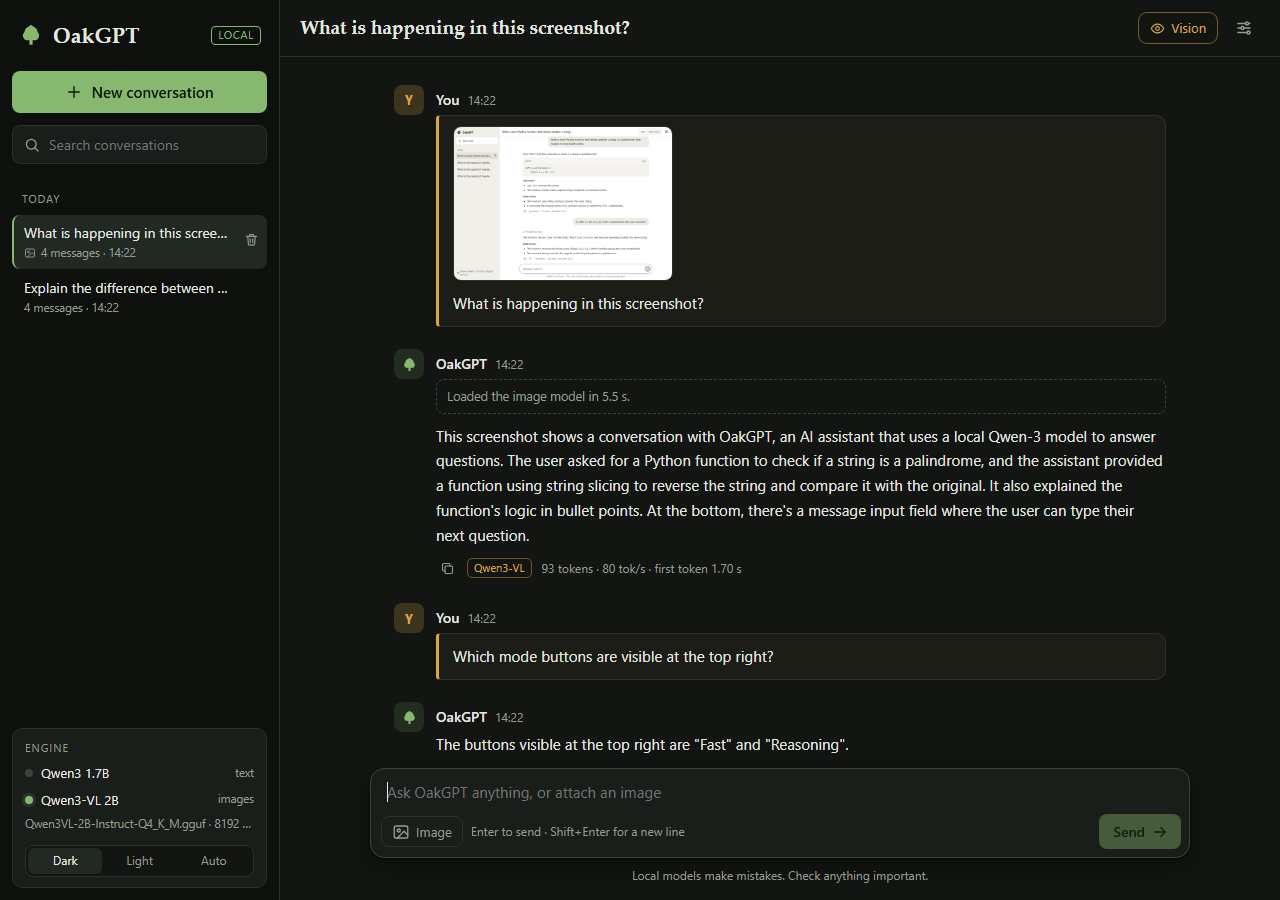
\includegraphics[width=0.8\textwidth]{figures/ui-vision-1280.png}
  \caption{An image conversation in the dark theme. The engine panel shows Qwen3-VL
    loaded. Values shown come from a demo session, not the study.}
  \label{fig:vision}
\end{figure}

\begin{figure}[H]
  \centering
  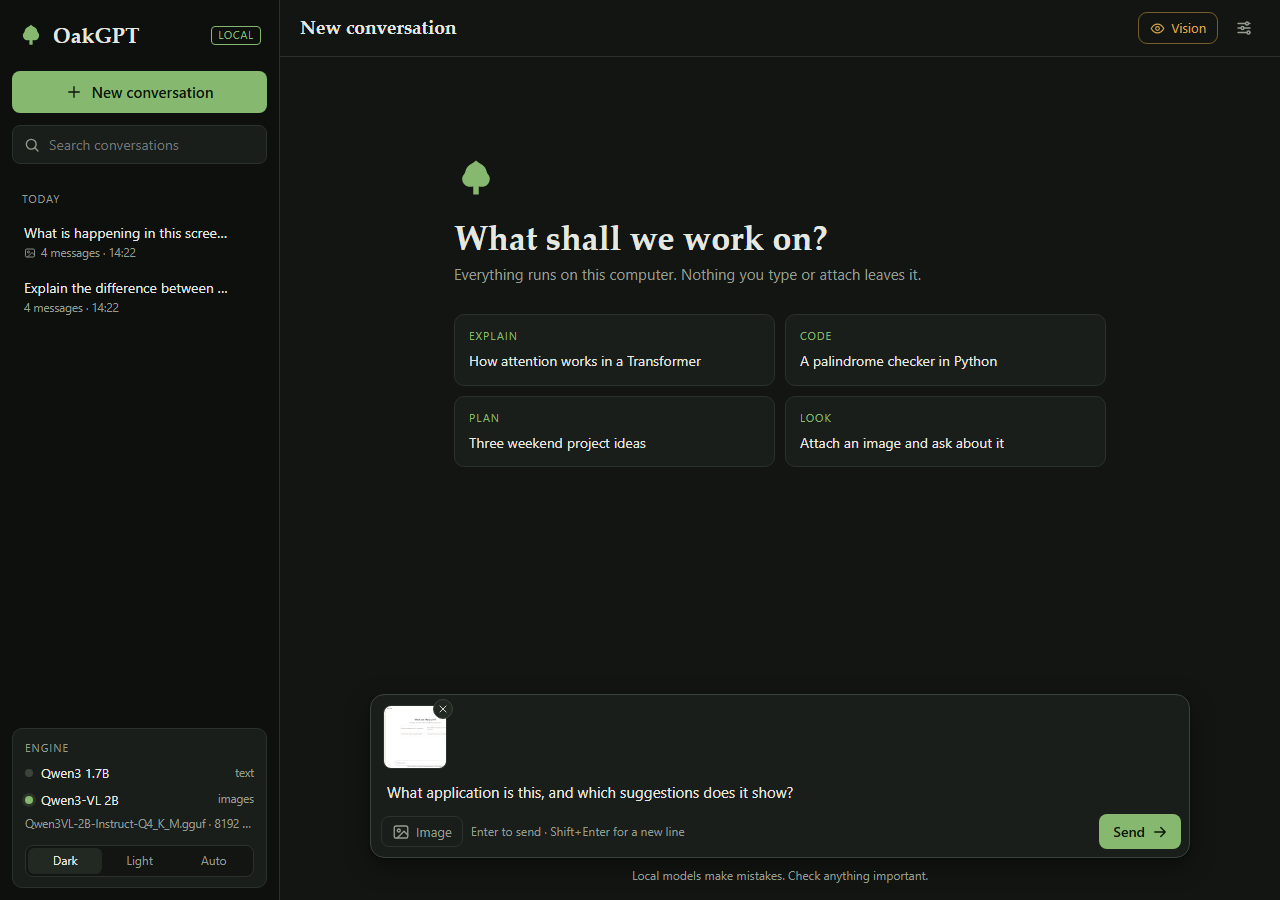
\includegraphics[width=0.8\textwidth]{figures/ui-composer-attachment-1280.png}
  \caption{An attachment preview in the composer; the mode switch has become the Vision
    badge.}
  \label{fig:composer}
\end{figure}

\begin{figure}[H]
  \centering
  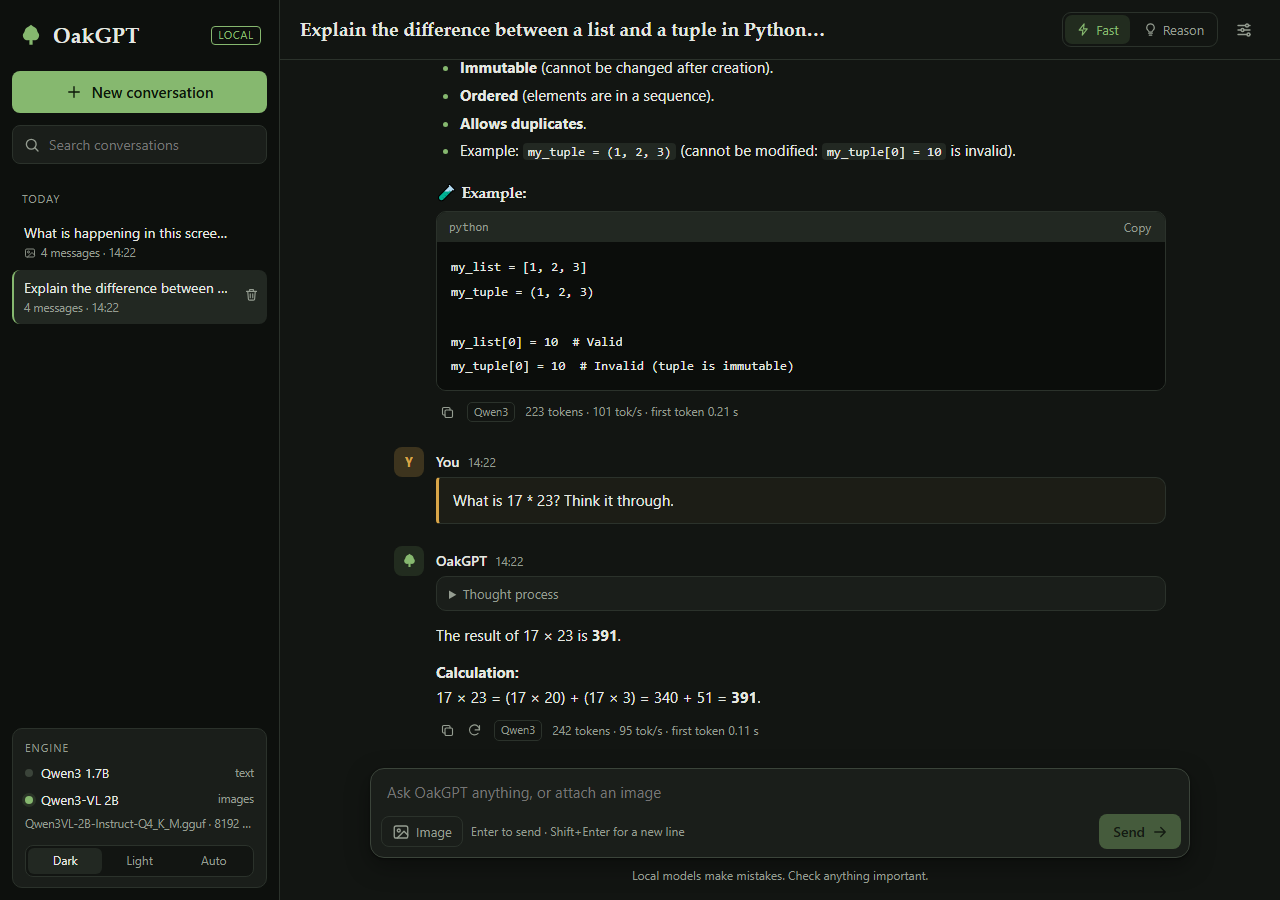
\includegraphics[width=0.8\textwidth]{figures/ui-text-1280.png}
  \caption{A text conversation on Qwen3 1.7B with code and a collapsed reasoning block.}
  \label{fig:text}
\end{figure}

\begin{figure}[H]
  \centering
  \begin{minipage}[b]{0.64\textwidth}
    \centering
    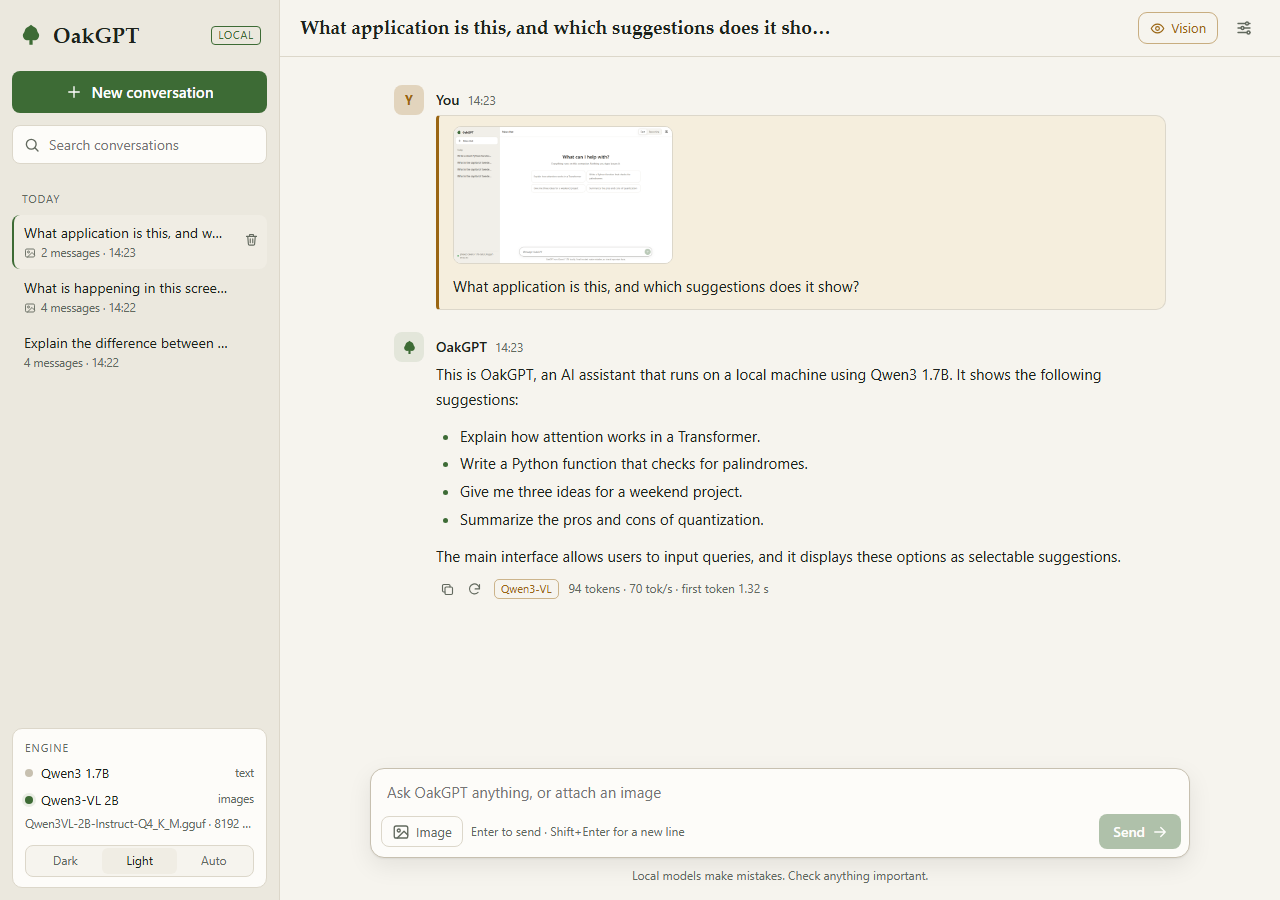
\includegraphics[width=\linewidth]{figures/ui-light-1280.png}
    \caption{Light theme.}
    \label{fig:light}
  \end{minipage}\hfill
  \begin{minipage}[b]{0.32\textwidth}
    \centering
    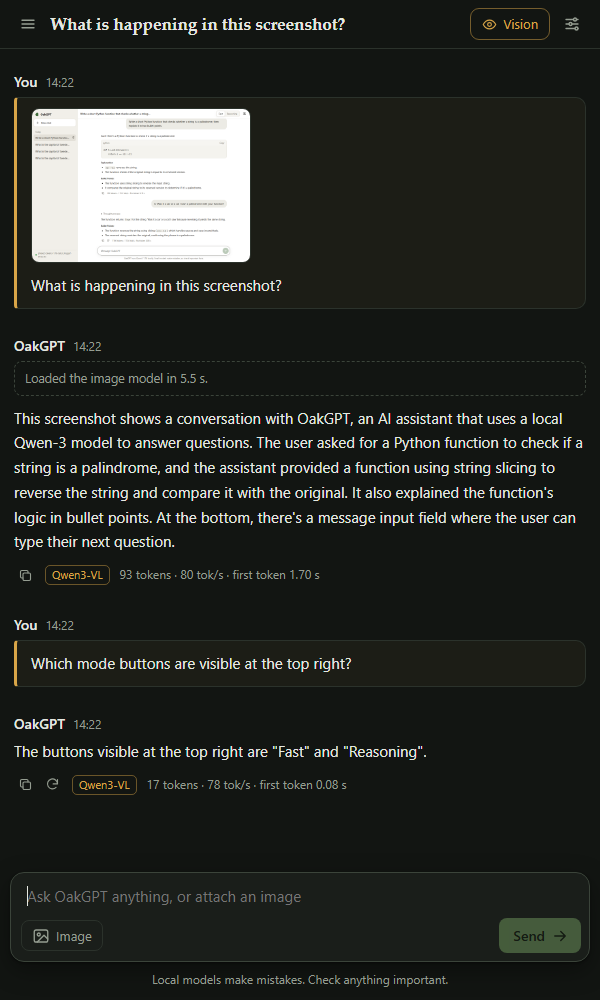
\includegraphics[width=\linewidth]{figures/ui-vision-narrow-600.png}
    \caption{Narrow layout, 600\,px.}
    \label{fig:narrow}
  \end{minipage}
\end{figure}

% ---------------------------------------------------------------------------
\section{Measured results (\code{vision\_study\_v1.json})}\label{sec:results}

\field{Design.} \path{scripts/measure_chat_vision.py} drove the running app over its HTTP
API (loopback only). The app had been restarted at commit \code{e5493c9}. The run had
four rounds:
\begin{itemize}
  \item \textbf{Images.} Rounds 0 and 2 used a 1280$\times$800 UI screenshot and asked a
        follow-up about it. Rounds 1 and 3 used a generated 640$\times$480 red-and-blue
        image.
  \item \textbf{Turns in each round:} a text turn, an image turn (forces a swap), the
        optional follow-up, and a text turn (swap back).
  \item \textbf{Decoding:} greedy, seed 2026, at most 160 new tokens.
  \item \textbf{Memory:} \code{nvidia-smi} sampled device-wide memory every 200\,ms (204
        samples).
\end{itemize}
The raw record contains the git revision (working tree dirty only through untracked
Phase 3.3 PDFs), the environment, the status before and after, every sample and every
turn.

\subsection{Model swaps}

\begin{center}
\small
\begin{tabular}{@{}lrrrrr@{}}
\toprule
Direction & Round 0 & Round 1 & Round 2 & Round 3 & Median \\
\midrule
text $\rightarrow$ vision (s) & 5.97 & 6.48 & 4.45 & 4.42 & 5.21 \\
vision $\rightarrow$ text (s) & 4.44 & 3.66 & 4.43 & 4.70 & 4.43 \\
\bottomrule
\end{tabular}
\end{center}

Each time covers process start until \code{/health} reports ok and the loaded model path
has been verified. A complete image reply including the swap took 5.6--8.4\,s of client
wall time.

\subsection{Image latency and cache reuse}

\begin{center}
\small
\begin{tabular}{@{}lrrr@{}}
\toprule
Turn & Image tokens & Server prompt ms & TTFT (s) \\
\midrule
Screenshot 1280$\times$800, cold & $\approx$1002 & 1484 / 1361 & 1.53 / 1.40 \\
Shapes 640$\times$480, cold & 302 & 718 / 740 & 0.73 / 0.76 \\
Follow-up on screenshot & 0 new; 1129 cached & 22 / 27 & 0.066 / 0.065 \\
\bottomrule
\end{tabular}
\end{center}

The prompt cache covers the image. The follow-up evaluated only 20 new tokens. Decode
rates were 77--96\,tok/s for Qwen3-VL and 81--102\,tok/s for Qwen3 in this run. A
swapped-in server starts with an empty cache: the text turns after a swap re-evaluated
their full prompt of 126--140 tokens in 187--230\,ms.

\subsection{Memory}

\begin{center}
\small
\begin{tabular}{@{}lr@{}}
\toprule
State & Device-wide \code{memory.used} \\
\midrule
No model loaded (during swaps) & 1085\,MiB minimum \\
Qwen3 1.7B, peaks per turn & 3203--3210\,MiB \\
Qwen3-VL 2B, peaks per turn & 4204--4281\,MiB \\
\bottomrule
\end{tabular}
\end{center}

This addresses the open C1 limitation about peak memory during generation for
Q4\_K\_M. At least 1.8\,GB stayed free at all times.

% ---------------------------------------------------------------------------
\section{Observed behaviour (single samples, not a benchmark)}\label{sec:observed}

\textbf{Correct:}
\begin{itemize}
  \item Asked about a screenshot of OakGPT, Qwen3-VL named the application and listed all
        four suggestion buttons word for word.
  \item It identified the ``Fast'' and ``Reasoning'' buttons.
  \item It described the generated image as a red background with a blue rectangle.
\end{itemize}

\textbf{Wrong:}
\begin{itemize}
  \item It placed the rectangle ``in the center''. The rectangle occupies the upper-left
        part of the image.
  \item Shown the C1 screenshot in which the text model wrongly claims that a palindrome
        check works, Qwen3-VL described the content correctly. It then judged the answer
        ``accurate and helpful''.
  \item Under greedy decoding, the text model said a GGUF file belongs to a ``Deep
        Learning Framework (DLT)'' related to DeepMind, which is a hallucination.
\end{itemize}

Across four rounds of greedy decoding, the text answer appeared in three different
wordings. This is consistent with the cache non-determinism documented in C1 (D9).

% ---------------------------------------------------------------------------
\section{Limitations and threats to validity}

\begin{itemize}
  \item \textbf{Quality.} Neither model's answer quality was evaluated.
        Section~\ref{sec:observed} contains single observations only.
  \item \textbf{Swap measurements.} One host, one run, four rounds and two images. Load
        times depend on disk cache state; the first swap after boot was not isolated.
  \item \textbf{Memory.} \code{nvidia-smi} reports device-wide usage, including the
        desktop. Sampling every 200\,ms can miss short peaks.
  \item \textbf{Browser.} Only Edge, headless, was tested. Drag and drop and paste were
        not automated. Accessibility beyond contrast was not audited, and widths below
        600\,px were not checked.
  \item \textbf{Security.} Prompt injection through text inside images is not mitigated
        (D19). A message containing control-token text cannot be sent in an image
        conversation; it is refused.
  \item \textbf{Exploratory probe.} The probe numbers in D18 and D20 (26.4\,s,
        974 tokens) come from a scratch run whose raw output was not archived.
\end{itemize}

% ---------------------------------------------------------------------------
\section{Next steps}

\begin{enumerate}
  \item \textbf{C2, fine-tuning}, with a frozen evaluation set first, as planned. A small
        image evaluation set (OCR, counting, colours, layout) would make D16--D21
        measurable.
  \item \textbf{Optional Thinking edition} of Qwen3-VL for image reasoning, measured
        against Instruct.
  \item \textbf{Choice of encoder precision.} Compare the Q8\_0 and F16 encoders in that
        evaluation before changing D17.
  \item \textbf{Browser coverage.} Automate drag and drop and paste in a browser test,
        and check widths below 600\,px.
\end{enumerate}

% ---------------------------------------------------------------------------
\section{Reproduction}

\begin{Verbatim}[fontsize=\footnotesize,frame=single,framesep=3mm]
.\.venv\Scripts\python scripts\fetch_vision_model.py   # pinned, SHA-256 verified
.\.venv\Scripts\oakgpt chat --config configs/chat/qwen3_q4km.json --no-browser
# In a second terminal (refuses to overwrite its output):
.\.venv\Scripts\python scripts\measure_chat_vision.py --rounds 4 `
    --output runs/chat/vision_study.json
# Live vision template test while the vision model is loaded:
$env:OAKGPT_VISION_URL = "http://127.0.0.1:18081"
.\.venv\Scripts\python -m pytest -m hardware -k vision_template
\end{Verbatim}

% ---------------------------------------------------------------------------
\begin{thebibliography}{7}
\small

\bibitem{c1} OakGPT Chat C1 report, decisions D1--D15: \path{reports/chat/c1/report.md}.

\bibitem{vlcard} Qwen Team, ``Qwen3-VL-2B-Instruct-GGUF'' model card, sections ``How to
  Use'' and ``Generation Hyperparameters,'' revision
  \code{52d6c8ffea26cc873ac5ad116f8631268d7eb503}, license apache-2.0.
  \url{https://huggingface.co/Qwen/Qwen3-VL-2B-Instruct-GGUF} (accessed 2026-11-23).

\bibitem{llamacpp} ggml-org, llama.cpp HTTP server README at commit
  \code{85cc432e2}: ``Multimodal support''; \code{prompt}
  input shapes and the note on \code{multimodal\_data}; options \code{--mmproj} and
  \code{--image-max-tokens}.
  \url{https://github.com/ggml-org/llama.cpp/blob/85cc432e2c8b92925f17dfb8937742541312f1d4/tools/server/README.md}

\bibitem{owaspllm} OWASP Gen AI Security Project, ``LLM01:2025 Prompt Injection,''
  Example Attack Scenario \#7 ``Multimodal Injection'' (``An attacker embeds a malicious
  prompt within an image that accompanies benign text'').
  \url{https://genai.owasp.org/llmrisk/llm01-prompt-injection/} (accessed 2026-11-23).

\bibitem{serverlog} llama-server b11930 startup log with
  \code{--mmproj mmproj-Qwen3VL-2B-Instruct-F16.gguf}, warning from \code{load\_hparams}
  (observed 2026-11-23; written to \path{runs/chat/server/<timestamp>/stderr.txt} on each
  managed start).

\bibitem{mdnimg} MDN Web Docs, ``Content-Security-Policy: img-src directive''
  (``specifies valid sources of images and favicons'').
  \url{https://developer.mozilla.org/en-US/docs/Web/HTTP/Reference/Headers/Content-Security-Policy/img-src}
  (accessed 2026-11-23).

\bibitem{wcag} W3C, ``Web Content Accessibility Guidelines (WCAG) 2.2,'' Success
  Criterion 1.4.3 Contrast (Minimum).
  \url{https://www.w3.org/TR/WCAG22/#contrast-minimum}

\end{thebibliography}

\end{document}
